\documentclass{lzureport}

\usepackage{caption}
\usepackage[dvipsnames]{xcolor}  % 更全的色系
\usepackage{listings}  % 排代码用的宏包

\usepackage{booktabs}

\usepackage{tabularx,array,makecell}
%\usepackage{color,xcolor}
%\usepackage{cases}
%\usepackage{mathtools}
%\usepackage{tcolorbox}
%\usepackage{tikz}
\usepackage{amsmath}
\usepackage{hyperref}

% 导言区
%\usepackage[round, sort]{natbib}
%\usepackage[authoryear]{natbib}

%%%%%%%%%%%%%%%%%%%%%%%%%%%%%%%%%%%%%%%%
%% listings设置
%%%%%%%%%%%%%%%%%%%%%%%%%%%%%%%%%%%%%%%%
\lstset{
	language = Python,
	backgroundcolor = \color{yellow!10},    % 背景色:淡黄
	basicstyle = \small\ttfamily,           % 基本样式 + 小号字体
	rulesepcolor= \color{gray},             % 代码块边框颜色
	breaklines = true,                  % 代码过长则换行
	numbers = left,                     % 行号在左侧显示
	numberstyle = \small,               % 行号字体
	keywordstyle = \color{blue},            % 关键字颜色
	commentstyle =\color{green!100},        % 注释颜色
	stringstyle = \color{red!100},          % 字符串颜色
	frame = shadowbox,                  % 用(带影子效果)方框框住代码块
	showspaces = false,                 % 不显示空格
	columns = fixed,                    % 字间距固定
	%escapeinside={<@}{@>}              % 特殊自定分隔符:<@可以自己加颜色@>
	morekeywords = {as},                % 自加新的关键字(必须前后都是空格)
	deletendkeywords = {compile}        % 删除内定关键字;删除错误标记的关键字用deletekeywords删!
}


\major{统计学}
\name{徐子扬}
\title{基因组学作业}
\stuid{320200904951}
\college{数学与统计学院}
\date{\zhtoday}
\expname{题目1-3}
\course{2023基因组学作业}

\begin{document}

\makecover

\begin{abstract}
    该作业报告完成了本学期基因组学课程布置的三道题目.
    
    作业第1题是“介绍Oxford Nanopore的原理、优缺点、应用”.对于原理,我主要介绍了该公司推出的首款纳米孔测序设备MinION\cite{2jain2016oxford}的技术原理,以及两种常见的Basecaller电流信号解码算法Nanocall\cite{david2017nanocall}和DeepNano\cite{bovza2017deepnano};
    对于优缺点,我讨论了长读长、高通量、实时靶向测序、直接检测碱基修饰等6种优点,以及准确性较低、高错误率等3种缺点,并与第一、二代测序进行比较;
    对于应用,我主要讨论了填补参考基因组中的空缺、建立新的参考基因组、识别大型结构变异等6种可能的应用场景.
    
    作业第2题是“简述我知道的RNA的种类和功能”.我简要概述了9种RNA的种类和功能.包括:mRNA(信使RNA)在基因表达过程中负责转导遗传信息;tRNA(转运RNA)在蛋白质合成过程中传递氨基酸;rRNA(核糖体RNA)作为核糖体的主要成分,参与蛋白质合成;snRNA(小核RNA)和snoRNA(小核仁RNA)参与RNA剪接和修饰;miRNA(微小RNA)调控基因表达,影响生物进程;lncRNA(长非编码RNA)在转录调控、基因沉默等方面发挥作用;piRNA(Piwi-interacting RNA)参与生殖细胞中的转座子沉默;circRNA(环状RNA)作为miRNA的海绵分子,调控基因表达.
    
    作业第3题是“泛基因组学(Pan-genome):内容、应用场景、研究实例”.对于内容,我主要介绍了泛基因组学的定义以及常见概念;对于应用场景,我给出作物基因组学、育种和进化研究、研究不同品种结构变异影响基因差异表达和结合GWAS数据捕获更完整的遗传变异信息共3种应用场景;对于研究实例,我选取了2023年3月在《Nature Communications》上发表的“亚洲水稻泛基因组倒位指数”文章《Pan-genome inversion index reveals evolutionary insights into the subpopulation structure of Asian rice》\cite{zhou2023pan},从研究背景、倒位指数、系统发育树、鉴定与评估等多个方面展开讨论,最后认为泛基因组学在大规模组学数据和科学计算时代可以发挥非常重要的作用.
    
    该作业使用LaTeX排版,编译所需的全部文件已经上传到\url{https://github.com/StatXzy7/lzu_genomics_hw}.
    
\end{abstract}

\textbf{关键词:} 基因组学; Oxford Nanopore; RNA; 泛基因组学
\newpage

\thispagestyle{empty}
\tableofcontents
\newpage 
\setcounter{page}{1}

\section{介绍Oxford Nanopore的原理、优缺点、应用}


牛津纳米孔技术Oxford Nanopore属于第三代DNA测序技术,其特点是单分子测序、实时测量和较长读长,从而大幅提升测序速度和准确性.英国的牛津纳米孔技术有限公司(Oxford Nanopore Technologies, ONT)专注于开发和销售纳米孔测序产品(如便携式DNA测序仪MinION,2014)\cite{1deamer2016three}\cite{2jain2016oxford},用于单分子的直接、电子分析.

自2014年提供首台纳米孔测序仪MinION以来,纳米孔测序技术及其在基础和应用研究中的应用得到了显著增长.纳米孔技术的快速发展带来了单个长DNA和RNA分子测序准确性、读长和吞吐量的大幅提升.为充分利用纳米孔长读长研究基因组、转录组、表观基因组和表观转录组,需要广泛发展实验和生物信息学方法.纳米孔测序应用于基因组组装、全长转录本检测、碱基修饰检测等领域,以及快速临床诊断和疫情监测等专门领域.通过开发新纳米孔、碱基调用方法和为特定应用定制实验方案,仍有数据质量和分析方法的问题值得改进.

\subsection{Oxford Nanopore牛津纳米孔测序技术的原理}

\subsubsection{Minion技术原理和测序步骤}
具体来说,我们这里主要讨论Oxford Nanopore推出的首款纳米孔测序设备MinION的技术原理.该技术依赖于纳米级蛋白质孔,即“纳米孔”,作为生物传感器,嵌入耐电性聚合物膜中.在电解液中,施加恒定电压产生流过纳米孔的离子电流,从而使带负电荷的单链DNA或RNA分子从带负电荷的顺式侧向带正电荷的反式侧穿过纳米孔.转移速率由一种马达蛋白控制,该马达蛋白以有序的方式推动核酸分子穿过纳米孔.在易位期间,离子电流的变化与感应区中的核苷酸序列相关,并利用计算算法进行解码,从而实现单分子的实时测序.除了控制转移速度外,马达蛋白还具有解旋酶活性,使双链DNA或RNA-DNA双链能够解离成通过纳米孔的单链分子.

\begin{figure}[htp!]
	\centering
	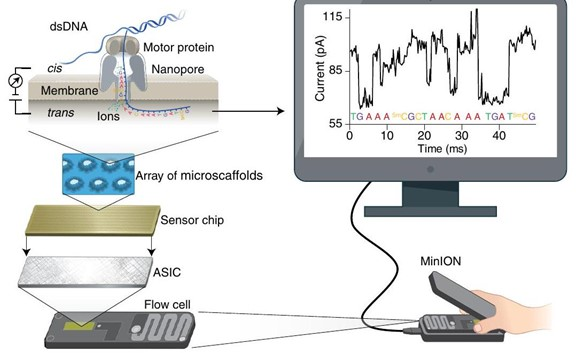
\includegraphics[width=0.8\linewidth]{figure/1mini}
	\caption{MinION nanopore sequencing 原理 \cite{0wang2021nanopore}} \label{MinION}
\end{figure}

图\ref{MinION}展示了MinION纳米孔测序原理.一个MinION Flow细胞包含512个通道,每个通道中有4个纳米孔,总计2,048个纳米孔用于DNA或RNA的测序.纳米孔位于由连接到传感器芯片的微支架阵列支撑的耐电聚合物膜内.每个通道与传感器芯片中的独立电极相连,并由专用集成电路(ASIC)单独控制和测量.由于在膜上施加了恒定电压,离子电流通过纳米孔,膜的反面带正电荷.在马达蛋白质的作用下,首先解开双链DNA(dsDNA)分子(或RNA-DNA杂交双链),然后在电压驱动下,单链DNA或带负电荷的RNA穿过纳米孔.当核苷酸通过纳米孔时,测量特征电流变化,并根据这些变化确定相应的核苷酸类型,每秒约可识别450个碱基(R9.4纳米孔).

原理中涉及到的主要概念和作用:
\begin{enumerate}
	\item 纳米孔:MinION设备包含众多纳米孔,嵌入一层类细胞膜物质(通常为生物膜蛋白).每个纳米孔可检测通过的DNA分子.
	\item 核酸分子穿孔:测序过程中,DNA分子被引导穿过纳米孔.需要对DNA分子进行处理,如加入适配器或线性化.
	\item 电压梯度与电流信号:纳米孔两侧施加电压梯度,使带负电荷的DNA分子受电场驱动穿过纳米孔.DNA分子穿过时,阻碍纳米孔内离子流,改变电流信号.电流信号随DNA中不同碱基(A、T、C和G)的通过而变化.
	\item 信号解码:MinION设备记录纳米孔实时电流信号,用专门算法将信号转换为对应碱基序列.
\end{enumerate}

图\ref{step}展示了DNA通过纳米孔转位的步骤:(i)开放通道;(ii)双链DNA(带有铅接头(蓝色)、结合分子马达(橙色)和发夹接头(红色))被纳米孔捕获;捕获后依次转位的是(iii)铅接头、(iv)模板链(金色)、(v)发夹接头、(vi)互补链(深蓝色)和(vii)拖尾接头(棕色);最后(viii)状态恢复至开放通道.在这个过程中,DNA以特定顺序穿过纳米孔,产生的离子电流信号可以被检测并用于解码DNA序列.

\begin{figure}[htp!]
	\centering
	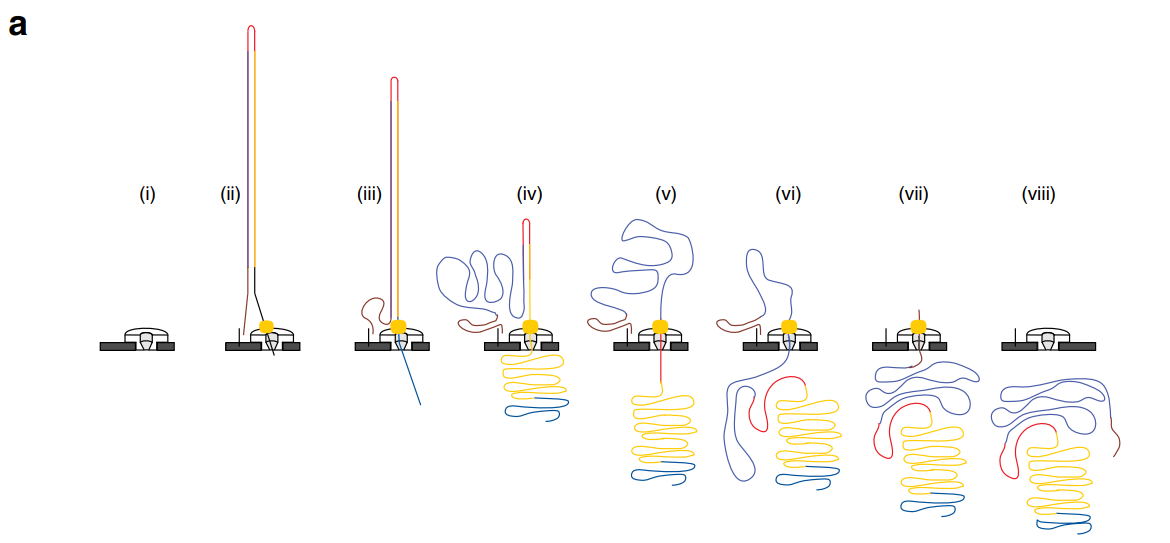
\includegraphics[width=0.8\linewidth]{figure/步骤}
	\caption{MinION nanopore sequencing 步骤 \cite{2jain2016oxford}} \label{step}
\end{figure}

\subsubsection{Basecaller电流信号解码算法}

当DNA分子穿过纳米孔时,不同的碱基(A、T、C和G)会引起电流信号的特异性变化.这些变化取决于每种碱基与纳米孔之间的相互作用,在实际情况中,单个碱基的信号解析很困难,因为测序过程中DNA是以k-mer(一般是3-6个连续碱基)的方式通过纳米孔的.因此,在实际应用中,通常会观察到由连续几个碱基组成的k-mer引起的复合信号.这些信号随着不同k-mer组合的通过而发生变化,可以通过特定的算法进行解码以获取原始的碱基序列.如何精确地将ONT生成的原始电信号翻译为序列信息(即basecalling)也就是科学家们关注的重点,当然也是我这个专业的研究者更关心的,所以还是得专门来讨论一下.


牛津纳米孔公司似乎提供了MinION的云计算服务Metrichor,该方法主要基于隐马尔可夫模型(HMM),但属于闭源软件.为了开发离线的替代方案,一些研究者着手研究开源算法,下面我们将主要讨论在文献\cite{2jain2016oxford}中提到的两种知名的算法Nanocall和DeepNano.

Nanocall\cite{david2017nanocall}是一种基于隐马尔可夫模型HMM的基本呼叫器Basecaller,它在本地执行高效的1D基本呼叫,无需互联网连接,其精度可与牛津纳米孔公司提供的基于Metrichor的1D基本呼叫相媲美.

Nanocall的输入是一组存储在ONT特定的FAST5文件中的分段事件序列.Nanocall分别处理每个输入文件,具体步骤如下.首先,在发现发夹结构时,将模板链和互补链分为单独的事件序列.接下来,它估算孔模型的缩放参数.可选地,Nanocall可以使用期望最大化算法进行多轮训练,以更新缩放参数,并使用标准的Baum-Welch算法\cite{baum1972inequality}更新状态转移参数.最后,Nanocall执行标准的Viterbi解码,以找到隐藏状态的路径,其中状态是纳米孔中的6-mer.对于上述模型中的一些经典算法,应当可以在任何一本随机过程或者生物信息学教材中找到,因此不再赘述.

具体地说,状态转移是从一个状态转移到另一个状态的先验概率.默认的状态转移是基于两个参数计算的:'stay'概率$p_{\text {stay }}$ 和'skip'概率$p_{\text {skip. }}$ 前者,$p_{\text {stay }}$,表示两个连续事件来自同一上下文/状态的概率.这对应于分割错误,即引入了错误的事件分割.后者,$p_{\text {skip }}$,表示两个连续事件来自状态差异超过一个kmer位移的概率.这对应于分割错误或测序错误(即DNA通过孔太快,无法捕捉可检测的事件events),其中一个或多个事件丢失.一个稍微复杂的问题是,通过增加跳过次数,总是有多种从一个状态到另一个状态的方式.例如,ACGTGT可以通过一次或三次跳过后在后面接上GTGTAC.下面对状态转移的计算也考虑到了这一点:
$$
\begin{aligned}
	\tau\left(k_1, k_2\right)= & \delta_{k_1=k_2} \cdot p_{\text {stay }} 
	 +\delta_{\text {suffix }\left(k_1, 5\right)=\operatorname{prefix}\left(k_2, 5\right)} \cdot p_{\text {step }} \cdot \frac{1}{4} \\
	& +\sum_{i=2}^5 \delta_{\text {suffix }\left(k_1, 6-i\right)=\operatorname{prefix}\left(k_2, 6-i\right)} \cdot p_{\text {skip } 1}{ }^{i-1} \cdot \frac{1}{4^i} 
	 +\sum_{i>5} p_{\text {skip } 1}{ }^{i-1} \cdot \frac{1}{4^6} .
\end{aligned}
$$
这里,$\delta$是标准示性函数;$\operatorname{prefix}(k, i) / \operatorname{suffix}(k, i)$是长度为$i$的$k$的前缀/后缀;$p_{\text {step }}:=\left(1-p_{\text {stay }}-p_{\text {skip }}\right)$;而$p_{\text {skip } 1}=p_{\text {skip }} /\left(1+p_{\text {skip }}\right)$对应恰好一个跳过的概率.


在包含隐状态的状态转移矩阵训练之后,Nanocall运行Viterbi解码算法,计算生成观察到的事件序列的最可能的状态序列.之后通过迭代添加在连续状态之间转换所需的最少碱基数来构建最终的碱基序列.例如,连续状态ACTCTC和CTCTCA生成碱基序列ACTCTCA,而不是ACTCTCTCA.特别地,由于这种启发式方法和纳米孔中不变状态的特性,所调用的碱基序列不会包含比kmer大小(6 bp)更长的同源重复序列.然而,仍能检测到长度大于1的重复序列.因此,Nanocall读取在大小为1的重复序列附近可能产生系统性(非随机)错误.

DeepNano\cite{bovza2017deepnano}是一个基于循环神经网络(recurrent neural network)\cite{giles1994dynamic}框架的算法,用于执行基调用,其精度优于基于HMM的方法.在互联网连接有限的情况下进行现场测序时,能够执行本地、离线基地呼叫非常有用.

在图\ref{deepnano}的DeepNano中,给定一组输入向量$\left\{\vec{x}_1, \vec{x}_2, \ldots, \vec{x}_t\right\}$.它的预测是一组输出向量$\left\{\vec{y}_1, \vec{y}_2, \ldots, \vec{y}_t\right\}$. 在这里,我们需要预测DNA序列,因此每个输入向量$\vec{x}_i$包含每个事件(即长度为k的电流信号)的均值、标准差和长度,输出向量$\vec{y}_i$给出了呼叫碱基的概率分布.
在处理每个输入向量$\vec{x}_i$时,循环神经网络计算两个向量:其隐藏状态$\vec{h}_i$和输出向量$\vec{y}_i$.这两者都取决于当前输入向量和之前的隐藏状态:$\vec{h}i=f\left(\vec{h}_{i-1}, \vec{x}_i\right), \vec{y}_i=g\left(\vec{h}_i\right)$.通常,通过使用具有多个隐藏层的神经网络可以提高预测准确性,其中每个层使用来自前一层的隐藏状态.我们使用具有三层或四层的网络.对于三层的计算如下:
$$
\begin{aligned}
	\vec{h}_i^{(1)} & =f_1\left(\vec{h}_{i-1}^{(1)}, \vec{x}_i\right) \\
	\vec{h}_i^{(2)} & =f_2\left(\vec{h}_{i-1}^{(2)}, \vec{h}_i^{(1)}\right) \\
	\vec{h}_i^{(3)} & =f_3\left(\vec{h}_{i-1}^{(3)}, \vec{h}_i^{(2)}\right) \\
	\vec{y}_i & =g\left(\vec{h}_i^{(3)}\right)
\end{aligned}
$$



\begin{figure}[htp!]
	\centering
	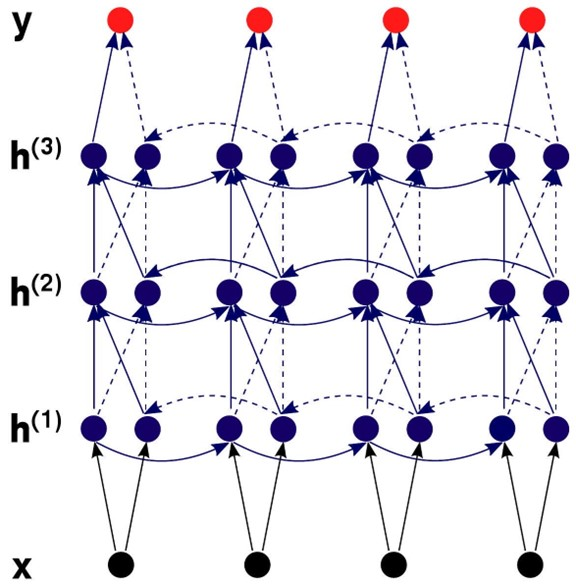
\includegraphics[width=0.8\linewidth]{figure/deepnano}
	\caption{deepnano 循环神经网络模型 \cite{bovza2017deepnano}} \label{deepnano}
\end{figure}



当然,对于上述两种算法循环神经网络和隐马尔可夫模型,实际上我个人认为两者的构造还是非常接近的,因为都存在相应的时序特征需要训练而且都共享训练权重,因此处理DNA序列肯定是有效的.不过如果现在让我设计的话,肯定是要加入预训练和Transformer模型了,时代在不断变化.




\subsubsection{原理总结}

Oxford Nanopore的纳米孔测序技术基于单个DNA分子通过纳米孔的电信号变化来实现.A、C、G、T 四种不同的碱基在电场作用下通过纳米孔时,会产生不同的电信号,这些信号可以被检测和记录下来.这些信号可以被转换成DNA序列,并且可以在实时中进行读取和分析.


\subsection{Oxford Nanopore牛津纳米孔测序技术的优缺点}

\subsubsection{优点}

\begin{enumerate}
	\item 长读长:
	纳米孔测序技术的长读长为DNA或RNA序列比对和匹配带来了优势,有助于获得高质量、更完整的基因组组装.长读长在植物基因组等具有复杂结构和高度重复区域的研究中显著,简化了从头组装过程,改进参考基因组,实现phasing,加快宏基因组物种鉴定.对于RNA,长读长有助于全长转录本表征,及异构体、剪接变体和融合转录本的量化和分析.由电检测提供的读长具有很高上限,依赖核酸转位物理过程,2018年实现了高达2.273兆碱基(Mb)的读长\cite{gong2019ultra}.
	
	\item 高通量:
	ONT测序技术具有较高吞吐量,满足不同项目规模需求.吞吐量提高得益于活跃纳米孔数量增加、DNA/RNA转移速度提升及运行时间延长.早期MinION用户报告每个流动池产量为数百兆碱基,而现吞吐量已增至约10-15千兆碱基(Gb),得益于更快的化学反应(R6纳米孔速度约每秒30个碱基,提高至R9.4纳米孔每秒约450个碱基)及引入Rev D SIC芯片后更长运行时间.后续设备,如PromethION,运行更多流动池,每个流动池纳米孔数量更多\cite{nicholls2019ultra}.
	
	
	\item 实时靶向测序:这是在短时间内获取和分析DNA或RNA序列的有效方法,尤其适用于临床应用.MinION平台因其小型、低成本、简易的文库准备和便携性,使实时分析成为可能\cite{loose2016real}.通过在测序过程中实时捕获和分析DNA链,可以迅速积累目标片段的读取.实时靶向测序技术有助于显著缩短从生物样本收集到数据分析所需的时间,对于现场和临床护理应用具有重要意义.
	
	\item 直接检测碱基修饰:第二代NGS技术无法直接检测原生DNA中的碱基修饰.然而,纳米孔技术可以对原生DNA和RNA的单个核苷酸进行单分子测序,从而检测其中的修饰.比如有研究发现,纳米孔系统能够准确识别五种不同类型的胞嘧啶\cite{wescoe2014nanopores}(包括C、5-甲基胞嘧啶、5-羟甲基胞嘧啶、5-甲酰胞嘧啶和5-羧胞嘧啶),准确率达92\%至98\%.
	
	\item 可直接对RNA表达分析:ONT技术可以直接测序RNA分子,提供更真实的转录本信息,避免了将RNA逆转录成cDNA的步骤.而NGS测序cDNA拷贝的片段较短,导致全长转录本的组装和RNA剪接异构体的准确表征困难.MinION平台可进行全长cDNA读取,例如研究利用MinION成功检测了果蝇中四个基因的RNA剪接变体和异构体,其中一个复杂基因的7000多种异构体的比对同一性高达90\%.这在450个碱基长度的NGS读取中是无法实现的\cite{bolisetty2015determining}.
	
	\item 便携性、简化性与低成本:ONT的便携设备如MinION和Flongle使纳米孔测序技术能在实验室之外的环境中使用,如现场实验和偏远地区.同时,ONT的测序流程无需PCR扩增,避免了PCR偏差和可能的错误.此外,ONT的设备和测序试剂价格相对较低,特别适合小规模实验和个体研究者.
	
\end{enumerate}


\subsubsection{缺点}

\begin{enumerate}
	
	\item 准确性较低:ONT纳米孔测序的一个主要缺点是其较低的测序准确性.与其他测序平台相比,ONT的单次读取准确性通常在85%-90%之间.这可能会影响某些应用,例如单核苷酸多态性(SNP)检测和低丰度变异体的识别.比如图\ref{miss}中显示的结果.
	
	\begin{figure}[htp!]
		\centering
		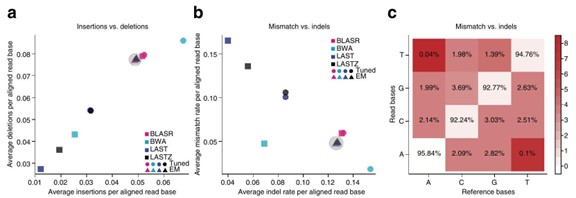
\includegraphics[width=1\linewidth]{figure/miss}
		\caption{MinION测序与参考序列比对结果\cite{2jain2016oxford}} \label{miss}
	\end{figure}
	
	\item 高错误率:ONT测序数据中的错误主要是插入和缺失错误,这可能会对某些应用产生负面影响,例如测序短的重复序列或串联重复序列.比如我们之前提到的Nanocall\cite{david2017nanocall}在大小为1的重复序列附近可能产生的系统性(非随机)错误.
	
	
	\item 数据分析难度大:由于测序产生的大量长读长数据而且还是电信号,数据分析需要较高的计算资源和专业知识,需要使用到比较先进的算法,比如我们之前提到的HMM,RNN,当然之后肯定还需要更先进的深度学习算法.
\end{enumerate}

\subsubsection{与第一、二代测序比较}


\begin{enumerate}
	\item 读长(Read Length):\\
	ONT测序技术可以生成非常长的读长(超过1 Mb),而第一代(例如Sanger测序)和第二代测序技术(例如Illumina)通常具有较短的读长(数百到数千个碱基).
	
	\item 准确性(Accuracy):\\
	ONT测序的准确性相对较低(约85%-90%),而Sanger测序的准确性高达99.99%,Illumina测序的准确性也在99%以上.
	
	\item 通量(Throughput):\\
	ONT测序通量适中,可以根据不同设备满足不同项目规模的需求.Illumina测序具有非常高的通量,适合大规模项目.而Sanger测序的通量相对较低.
	
	\item 实时性(Real-time):\\
	ONT测序技术具有实时分析的能力,可以在测序进行时获取数据.而Sanger测序和Illumina测序在完成整个测序过程后才能获取数据.
	
	\item 样品准备(Sample Preparation):\\
	ONT测序通常不需要PCR扩增,可以避免引入PCR偏差和可能的错误.而Sanger测序和Illumina测序通常需要进行PCR扩增.
	
	\item 成本(Cost):\\
	ONT测序设备和试剂相对较便宜,尤其适合小规模实验和个体研究者.Sanger测序成本适中,但通量较低.Illumina测序在大规模项目中成本效益较高,但对于小规模实验成本可能较高.
	
	\item 便携性(Portability):\\
	ONT的设备(如MinION和Flongle)非常小巧便携,适合现场实验和远程地区.而Sanger测序和Illumina测序设备较大,通常需要固定在实验室中使用.
\end{enumerate}

\subsection{Oxford Nanopore牛津纳米孔测序技术的应用}
    牛津纳米孔测序技术在基础研究、临床应用和现场应用等领域有着广泛的应用.这些应用根据ONT测序的优势,如长读长、原生单分子和便携性等特点,可以进一步细分为多个具体主题.

\begin{figure}[htp!]
	\centering
	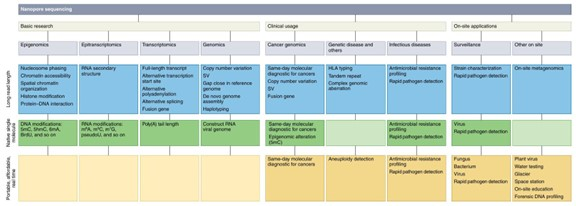
\includegraphics[width=1\linewidth]{figure/ontapp}
	\caption{Oxford Nanopore牛津纳米孔测序技术的应用表 \cite{0wang2021nanopore} } \label{ontapp}
\end{figure}

\subsubsection{填补参考基因组中的空缺}

牛津纳米孔测序技术在基因组组装方面具有显著应用价值,特别是在填补参考基因组中的空缺和识别重复区域方面.人类基因组、线虫参考基因组等已经通过ONT长读长成功地填补了空缺和扩展.在其他模式生物、近缘物种和非模式生物方面也取得了类似的进展,有助于改善这些物种基因组的连续性和完整性.例如,ONT读取已用于关闭人类参考基因组中的12个缺口(每个缺口> 50 kb),测量端粒重复的长度,以及组装人类Y染色体的中心粒区域\cite{jain2018linear}.此外,ONT使得首次实现了人类X染色体的无缺口端粒至端粒组装,包括重建约2.8 Mb的中心粒卫星DNA阵列和关闭所有剩余的29个缺口(总计1.1 Mb)\cite{miga2020telomere}.

\subsubsection{建立新的参考基因组}

牛津纳米孔测序技术在非模式生物初始参考基因组的组装中发挥了重要作用.例如,通过仅使用ONT数据或结合其他技术,成功组装了根腐病菌、澳大利亚最大淡水鱼、普通小丑鱼等物种的基因组.ONT直接RNA测序也被用于构建RNA病毒基因组,无需传统的反转录步骤.在SARS-CoV-2大流行期间,ONT测序通过cDNA和直接RNA测序重建了全长SARS-CoV-2基因组序列,为病毒的生物学、进化和致病性研究提供了重要信息.

\subsubsection{识别大型结构变异(SV)}

牛津纳米孔测序技术在识别大型结构变异方面具有显著优势,特别是在生物医学背景中.例如,它已成功应用于乳腺癌细胞系、急性髓系白血病患者以及具有先天异常的个体.ONT技术还有助于在人类基因组中识别大量结构变异.

\subsubsection{表征全长转录组和复杂转录事件}

ONT cDNA测序技术在表征全长转录组和复杂转录事件方面展现了显著的潜力.与PacBio长读长相比,它在识别基因亚型方面具有相似的性能.虽然在评估基因丰度和检测剪接位点方面存在一定的限制,但准确性和吞吐量的改进正在改善这些分析.ONT技术还用于研究不同生物中的RNA分子的poly(A)尾长以及人类环状RNA的全长亚型.

\subsubsection{检测RNA修饰}

ONT直接RNA测序技术为检测具有关键生物学功能的RNA修饰和RNA编辑提供了新的可能性.通过ONT测序,研究者在不同生物中检测了各种RNA修饰\cite{garalde2018highly},如m6A、m7G和假尿苷.此外,结合人工化学修饰,ONT直接RNA测序可以用于探测RNA的二级结构.同时,通过标记新生RNA并进行ONT直接RNA测序,RNA代谢动态也得到了分析.

\subsubsection{癌症研究治疗}

ONT测序技术已广泛应用于各种癌症类型,以识别复杂的基因组变异.这种技术可以快速检测白血病患者中的突变、染色体易位和断点.同时,ONT测序还能分析具有高重复序列和大基因大小的癌症易感基因.通过直接检测DNA修饰\cite{euskirchen2017same},ONT数据可同时捕获基因组和表观基因组变异.ONT测序技术还可以在短时间内为癌症提供多模式的快速分子诊断.例如,它已成功应用于检测临床样本中的融合基因\cite{jeck2019nanopore}.总之,ONT测序技术在癌症研究中具有显著的应用价值,为更深入地了解癌症相关基因突变和诊断提供了有力工具.

\section{简述我知道的RNA的种类和功能}

在生物学中,RNA(核糖核酸)是一类具有多种功能的生物大分子,涉及基因表达调控、蛋白质合成和基因组稳定等重要生物过程.了解RNA的种类和功能对于深入理解生物学的基本原理和各种生命活动至关重要.许多教材和专著都详细描述了不同类型的RNA及其作用,而本章节将简要介绍我所知道的所有RNA种类及其功能.我的回答主要参考了教材\cite{2019基因组学},并结合了其他相关资料.

\subsection{mRNA(信使RNA)}
mRNA(信使RNA)在基因表达过程中发挥着关键作用,负责将DNA中的遗传信息传递到蛋白质.mRNA的生成、加工和翻译调控是生物学中基因表达调控的核心环节.

在生物学定义上,mRNA是DNA和蛋白质之间的信息传递桥梁.DNA中的基因在转录过程中被转录成mRNA,mRNA携带着来自DNA的遗传信息.这一过程由RNA聚合酶催化完成,生成初始的前mRNA.

在功能上,mRNA经过一系列修饰和加工,如5'帽子添加、3'尾部加多聚腺苷酸(Poly-A)尾、选择性剪接等,形成成熟的mRNA.这些修饰有助于mRNA的稳定性和翻译效率,同时影响mRNA在细胞内的定位和运输.

在生物学过程中,mRNA从细胞核转移到细胞质,在核糖体上进行翻译,指导蛋白质的合成.核糖体依次识别mRNA上的密码子,tRNA携带对应的氨基酸与mRNA的密码子配对,逐渐将氨基酸连接成蛋白质链.
不同物种和生物过程中的mRNA表达受到多层次的调控.如转录后调控(mRNA降解、局部翻译等)、非编码RNA(如miRNA)的作用等,这些调控机制共同影响蛋白质的合成和细胞功能.


\subsection{tRNA(转运RNA)}
tRNA(转运RNA)是蛋白质合成过程中的核心组成部分,它负责将特定的氨基酸带到核糖体上,并与mRNA上的密码子配对,实现遗传信息的解码和蛋白质合成的指导.

在生物学定义上,tRNA是一类小分子RNA,其具有独特且高度保守的二级结构,称为“三叶草”结构.这一结构具有抗核酸酶降解的稳定性,并使得tRNA能够在不同物种中起到相似的功能.tRNA的一个端部携带氨基酸,而另一端包含一个与mRNA密码子互补的反密码子.

在功能上,tRNA的主要作用是在蛋白质合成过程中将氨基酸带到核糖体上.在翻译过程中,核糖体会读取mRNA上的遗传密码,tRNA的反密码子与mRNA上的密码子进行互补配对,将相应的氨基酸带到核糖体上,从而将氨基酸连接成蛋白质链.

在生物学过程中,tRNA的作用对生物的生长、发育和生存至关重要.通过将氨基酸正确地带到核糖体上,tRNA使得蛋白质能够按照mRNA上的遗传密码正确地合成,从而保证了生物体的正常生理功能.例如,在人类肌肉细胞中,tRNA对肌纤维蛋白的合成起着关键作用,影响着肌肉的功能和力量.



\subsection{rRNA(核糖体RNA)}
核糖体RNA(rRNA)在生物体内具有重要的功能.它是核糖体的主要组成成分,起到关键作用,确保生物体内蛋白质合成过程的顺利进行.

在生物学定义上,rRNA是一类非编码RNA,不参与蛋白质的编码过程,但在细胞功能中起着至关重要的作用.rRNA分子具有一定的保守性,这使得它们在不同物种中能够发挥相似的功能.核糖体是生物体内进行蛋白质合成的场所,负责将遗传信息从mRNA转化为蛋白质.在核糖体中,rRNA与蛋白质共同组成核糖体的亚基,参与蛋白质合成的关键步骤.

在功能层面,rRNA在核糖体结构和功能中发挥核心作用.它参与蛋白质合成过程中的多个关键步骤,如mRNA的辨认、tRNA的结合以及肽键的形成等.例如,在核糖体的A位、P位和E位上,rRNA与tRNA形成稳定的相互作用,确保氨基酸被正确地添加到生长中的肽链上.此外,rRNA在肽链延长和终止阶段也发挥作用,促使新合成的蛋白质从核糖体中释放.

rRNA对于生物的生长、发育和生存具有重要意义.核糖体数量和活性与生物体的生长速度密切相关,而rRNA的合成和稳定性是核糖体生物合成的关键因素.在一些疾病中,如核糖体功能障碍症,rRNA的异常表达或处理可能导致细胞功能障碍和发育异常.


\subsection{snRNA(小核RNA)}
snRNA是长度在20到300个核苷酸之间的小分子RNA,在生物学中具有重要功能.snRNA与蛋白质结合,形成剪接体,参与mRNA剪接过程.

在真核生物中,剪接是mRNA成熟过程中的一个关键环节.在该过程中,mRNA中的内含子(非编码区)被去除,而外显子(编码区)被连接在一起,形成成熟的mRNA.这个过程的正确进行是蛋白质合成和基因表达的关键.snRNA分子与蛋白质结合形成剪接复合物,参与识别和移除内含子,从而使mRNA正确剪接.

\subsection{snoRNA(小核仁RNA)}
snoRNA是长度在60到300个核苷酸之间的小分子RNA,在生物学中发挥关键作用.主要参与rRNA和tRNA的化学修饰,如2'-O-甲基化和假尿苷化等.

snoRNA通过与蛋白质结合,形成核仁小颗粒(snoRNP),在rRNA和tRNA的修饰过程中起作用.例如,在酵母中,U14 snoRNA参与18S rRNA的加工过程,对核糖体的生物合成具有关键作用.snoRNA与rRNA和tRNA中特定位点互补配对,引导相关酶进行正确的化学修饰.

\subsection{miRNA(微小RNA)}
miRNA是长度约为22个核苷酸的非编码RNA,在生物学中具有重要功能.通过与mRNA的3'非翻译区域(3' UTR)结合,调控基因表达,影响生长、分化和凋亡等细胞过程.

miRNA的生物合成包括pri-miRNA的转录、剪切生成pre-miRNA和加工成成熟miRNA.成熟的miRNA与RNA诱导沉默复合体(RISC)结合,与目标mRNA完全或部分互补配对,导致mRNA降解或翻译抑制,从而调控基因表达.

miRNA在生物学过程中发挥关键作用,调控基因表达具有重要意义.例如,miR-34家族在哺乳动物中发挥抗肿瘤作用,通过抑制细胞生长和促进细胞凋亡来抑制肿瘤发生.这些调控机制对维持生物体内稳态及响应环境变化至关重要.

\subsection{lncRNA(长非编码RNA)}
lncRNA是长度超过200个核苷酸的非编码RNA.与mRNA不同,它们不直接参与蛋白质合成.然而,在基因调控、染色质修饰和X染色体失活等方面,lncRNA具有多种功能.

作为基因调控因子,lncRNA可以在转录和翻译水平上调控基因表达.例如,HOTAIR通过与PRC2互作,在染色质上引导H3K27me3修饰,抑制靶基因表达.此外,lncRNA还可作为"miRNA海绵",调节miRNA对靶基因的调控.

在染色质修饰方面,lncRNA参与组蛋白修饰,影响染色质状态.例如,Xist与X染色体失活过程密切相关.在雌性哺乳动物中,Xist通过与染色质修饰因子相互作用,导致一个X染色体的失活,平衡雌性与雄性之间X染色体上基因的剂量.

\subsection{piRNA(Piwi-interacting RNA)}
piRNA是与Piwi家族蛋白结合的小分子RNA,长度约为26-31个核苷酸.piRNA主要在生殖细胞中发现,参与转座子沉默和基因调控.

piRNA与Piwi蛋白结合,形成piRNA-Piwi复合物,起到转座子沉默作用.转座子是可在基因组内移动的遗传元素,它们的不受控制的活动可能导致基因突变和基因组不稳定.piRNA通过引导piRNA-Piwi复合物结合到转座子的转录物,阻止其转录和复制,维护生殖细胞基因组的稳定性.

除转座子沉默作用外,piRNA还参与基因表达调控.在果蝇中,piRNA可以引导piRNA-Piwi复合物结合到mRNA分子,导致mRNA的降解,影响基因表达.此外,piRNA还参与染色质修饰.

\subsection{circRNA(环状RNA)}
circRNA是一类环形结构的非编码RNA,长度可变,通常比线性RNA更加稳定.它们在生物学中具有多种功能,如基因表达调控、作为miRNA的海绵和编码蛋白质等.

circRNA可以调控基因表达.一些circRNA通过与转录因子结合,影响转录因子的活性,进而调节基因的转录.此外,circRNA还可以与RNA结合蛋白相互作用,影响mRNA的加工和稳定性.尽管circRNA主要被认为是非编码RNA,但一些circRNA具有编码蛋白质的潜能.这些circRNA包含开放阅读框(ORF),在特定条件下,可通过转录和翻译产生蛋白质,从而影响生物学过程.



\section{泛基因组学(Pan-genome):内容、应用场景、研究实例}
泛基因组代表了一个物种内的所有基因集合,由核心基因组(包含物种所有个体间共享的序列)和“可选”基因组组成.2005年,泛基因组这一概念首次应用于细菌物种研究\cite{tettelin2005genome},当时在对数株链球菌(Streptococcus agalactiae)的测序中发现,核心基因组包含了80\%的链球菌基因,而其余20\%的基因在至少一个菌株中缺失.从那时起,研究人员一直在努力揭示许多物种的泛基因组,如2010年进行的人类泛基因组研究\cite{li2009human}.泛基因组研究表明,依赖于单一的参考基因组可能会对我们对物种多样性的理解产生负面影响.例如,在植物物种中\cite{Bayer2020PlantPA},与农艺性状相关的许多重要基因通常位于可选基因组中.随着基因组测序技术的不断改进,特别是长读取测序的发展,研究者们开始构建更复杂物种的泛基因组.通过泛基因组研究,我们发现单一参考基因组无法充分代表物种内群体的遗传多样性,因此泛基因组研究在未来植物育种、疾病抗性和环境适应性等方面具有广泛的应用前景.

\subsection{内容}
泛基因组(pangenome 或 supragenome)是指分类单元(clade)内所有菌株(strains, 实际上也可以推广到物种)的所有基因集合.它可分为核心泛基因组(core pangenome,所有个体中存在的基因)、壳层泛基因组(shell pangenome,两个或更多菌株中存在的基因)和云泛基因组(cloud pangenome,仅在单个菌株中发现的基因),如图\ref{Parts_of_the_pangenome}中所示.云基因组也称为附属基因组,包含部分菌株中存在的可有可无的基因和菌株特异性基因.研究泛基因组的领域称为泛基因组学.

\begin{figure}[htp!]
	\centering
	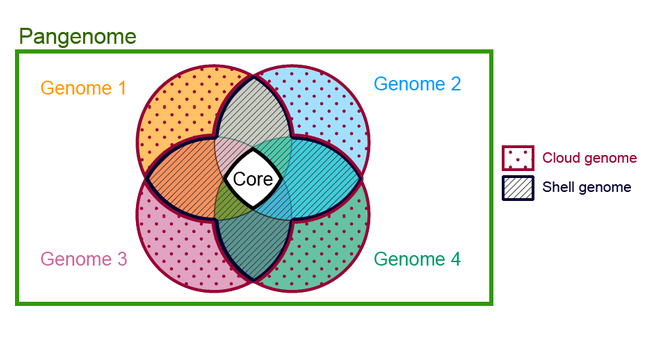
\includegraphics[width=1\linewidth]{figure/Parts_of_the_pangenome}
	\caption{泛基因组中的不同类型} \label{Parts_of_the_pangenome}
\end{figure}


细菌物种的基因组比单个菌株的基因含量大得多.有些物种具有开放泛基因组,而另一些具有封闭泛基因组.人口规模和生态位多样性被认为是决定泛基因组大小的主要因素.
泛基因组最初为细菌和古菌物种构建,近年来发展了真核生物泛基因组,特别是植物物种.泛基因组动态与可移动元件有关,具有重要的进化背景意义,与宏基因组学相关,也在更广泛的基因组学背景中使用.


\begin{figure}[htp!]
	\centering
	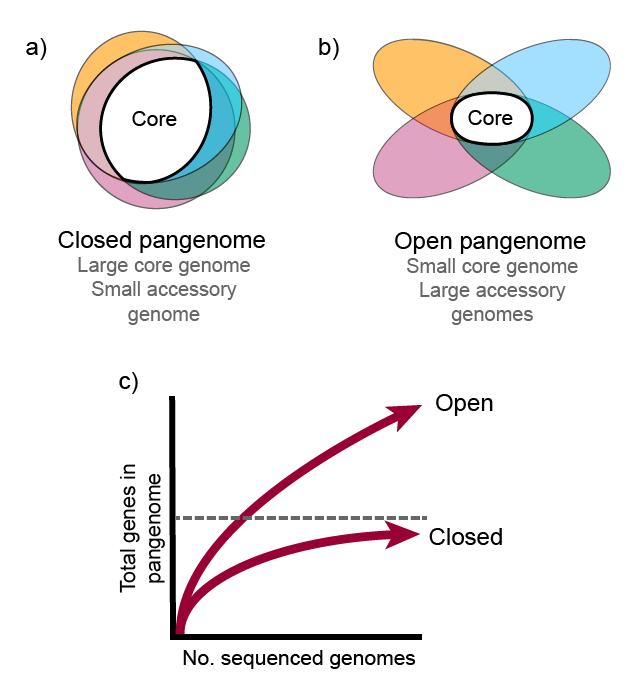
\includegraphics[width=0.55\linewidth]{figure/open_close}
	\caption{封闭和开放泛基因组.封闭泛基因组趋于渐近,可以预测完整大小.} \label{open_close}
\end{figure}

\subsection{应用场景}

想要深入理解泛基因组学的应用场景首先得明白泛基因组学的优点.泛基因组学的优点在于它能够更全面地揭示物种内的基因组多样性,揭示了整个基因组在不同物种中的重要性.因此,泛基因组学为我们提供了一个更全面的视角来研究物种内的遗传多样性,并为发掘有益基因提供了丰富的资源.



\subsubsection{作物基因组学、育种和进化研究}

泛基因组可以支持植物育种和进化研究,探讨基因存在和缺失变异的起源.第一个植物泛基因组研究是基于七个野生大豆个体的全基因组对比,发现与种子成分、开花和成熟时间、器官大小和生物量相关的可变基因以及在野生大豆Glycine soja中存在、而在家养大豆Glycine max中不存在的病害抗性基因\cite{li2014novo}.另一个研究基于三个不同水稻品种,发现一个栽培品种中S5杂种不育座位的缺失以及Sub1A水生状耐受基因的PAV\cite{schatz2014whole}.

\subsubsection{研究不同品种结构变异影响基因差异表达}

结构变异会影响基因的转录调控和表达,例如基因剂量变化、可变剪接和转录调控因子结合位点的改变.大豆泛基因组研究中,研究者通过对26个具有代表性的野生和栽培大豆品种进行de novo基因组组装,构建了一个高质量的基于图的大豆泛基因组.这一研究揭示了许多通过短序列直接映射到单一参考基因组上难以发现的遗传变异.基于图谱基因组的2,898个加入物的结构变异和来自代表性的26个加入物的RNA测序(RNA-seq)数据有助于将遗传变异与负责重要性状的候选基因联系起来.这一泛基因组资源将促进大豆的进化和功能基因组学研究.\cite{liu2020pan}.

\subsubsection{结合GWAS数据捕获更完整的遗传变异信息}

通过将泛基因组应用于GWAS分析,研究人员可以更全面地了解植物基因组的多样性,从而有助于揭示与重要性状相关的遗传变异,推动植物遗传改良和功能基因组学研究.传统GWAS分析在缺失参考基因组中的功能基因时,可能无法准确关联表型.然而,采用泛基因组作为参考,将结构变异纳入GWAS分析,有助于解决这一问题.

以一项关于油菜(Brassica napus)的研究\cite{song2020eight}为例,研究者通过测序、de novo组装和注释8个油菜品种,揭示了大量小型变异和存在及缺失变异(PAV).PAV基因组广泛关联研究(PAV-GWAS)成功确定了与籽荚长度、种子重量和开花时间相关的因果结构变异,这些变异在基于单核苷酸多态性的GWAS(SNP-GWAS)中未被检测到.此研究表明,PAV-GWAS可补充SNP-GWAS,识别与性状相关的关联,并为深入了解油菜基因组结构和遗传改良提供资源.

\subsection{研究实例:亚洲稻米泛基因组倒位指数}
下面,我将介绍一篇关于亚洲稻米泛基因组学研究的文章.这篇文章于2023年3月发表在《Nature Communications》上,题目为“亚洲水稻亚种群结构中泛基因组倒位指数揭示的进化启示”(Pan-genome inversion index reveals evolutionary insights into the subpopulation structure of Asian rice)\cite{zhou2023pan}.本文的主要作者是Yong Zhou等人,来自KAUST等多个机构.这项研究旨在探索亚洲稻米的基因多样性,并通过泛基因组学方法提供进化方面的见解.

\subsubsection{研究背景和内容}

为了应对2060年至2070年预期将达到100亿的全球人口增长,稻米研究社区正寻求创新方法,培育出营养丰富、可持续、能适应气候变化的新品种.在亚洲稻米的基因组中,有一些基因片段的顺序与其他个体不同,这种现象被称为倒位(inversion)\cite{rice}.倒位是一种重要的基因组结构变异,它可以影响基因的表达和功能.

本研究使用了73个高质量亚洲水稻(Oryza sativa)基因组,覆盖其亚种群结构,以及2个野生近缘种(O. rufipogon和O. punctata).研究人员基于这些基因组构建了一个包含1769个非冗余倒位的泛基因组倒位指数,涵盖了约29%的O. sativa cv. Nipponbare参考基因组序列.

通过该倒位指数,研究者估计亚洲水稻倒位发生率约为每百万年700次,这一速率是以往植物研究估算的16至50倍.对这些倒位的详细分析表明,它们对基因表达、重组率和连锁不平衡具有显著影响.该研究揭示了亚洲水稻泛基因组中大型倒位(≥100 bp)的普遍性和规模,并暗示了其在功能生物学和作物性状方面尚未充分研究的潜在影响.

\subsubsection{水稻倒位指数概述}

图\ref{invsum}中,$\mathbf{a}, \mathbf{b}$ 代表重采样置换检验,用于确定基因组数量与所有倒位和非基因组特异性倒位之间的关系;$ \mathbf{c} $ 倒位区域密度;$ \mathbf{d} $ Bionano对大于1 Mb的倒位进行验证,即Clu-INV0100180,Clu-INV0100660和Clu-INV0600550.在每个面板中,顶部线条显示作为参考的光学图谱,底部线条显示具有倒位的品种的基因组组装.灰色线条连接对齐的限制位点(蓝色区域),而黄色片段显示未对齐区域.黑色框突出显示每个倒位的位置.源数据作为源数据文件提供.

\begin{figure}[htp!]
	\centering
	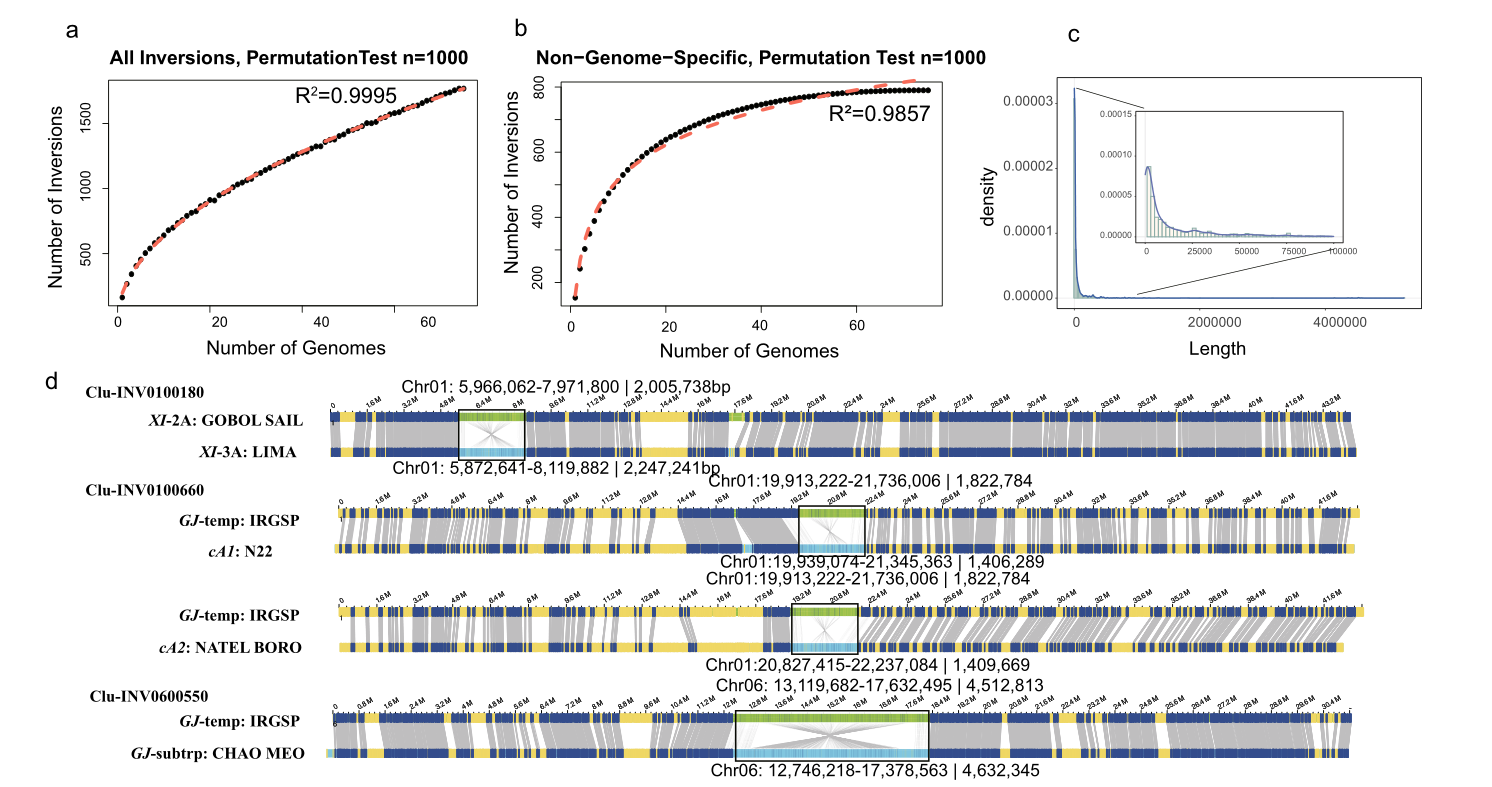
\includegraphics[width=1\linewidth]{figure/invsum}
	\caption{水稻倒位指数概述图} \label{invsum}
\end{figure}

这部分中,研究人员使用了一些典型的数据处理方法:

\begin{enumerate}
	\item 重采样置换检验(Resampling permutation test):这是一种统计方法,通过对数据进行随机重新排列,来评估观察到的结果是否具有显著性.在本研究中,研究者使用重采样置换检验来确定基因组数量与所有倒位和非基因组特异性倒位之间的关系.
	
	在 $ n $ 次置换后,对于重采样置换检验的 $ p $ 值计算可使用以下公式:
	$$
	p=\frac{1+\sum_{i=1}^n I\left(T_i \geq T_{o b s}\right)}{n+1}
	$$
	其中, $I$ 是示性函数,$ T_i $ 表示第 $ i $ 次置换的统计 量,$T_{obs}$表示观察到的统计量,$ n $表示置换次数.
	
	\item 倒位区域密度(Density of inversion regions):这是一种用于描述倒位在基因组上分布密度的指标.通过计算倒位区域的密度,研究者可以更好地了解倒位在水稻基因组中的分布特征.
	
	为了估计亚洲稻基因组倒位率(IR),本文考虑了具有最近共同祖先(MRCA)分歧时间估计的种群或基因组对,并将倒位总数除以两倍的最近共同祖先时间(TMRCA,对应于两个节点上的谱系总分支长度),即使用以下方程计算估计值:
	
	$$
	I R=\frac{N u m b e r \text { of } I N V s}{2 \times T M R C A}
	$$
	
	\item Bionano验证:Bionano是一种基于光学映射技术的基因组结构变异检测方法.本研究中,研究者使用Bionano技术验证了大于1 Mb的倒位,以确保倒位检测结果的准确性.在图中,顶部线条显示作为参考的光学图谱,底部线条显示具有倒位的品种的基因组组装.通过比较这些数据,可以直观地了解倒位的位置和特征.
\end{enumerate}

\subsubsection{系统发育树分析}

使用全基因组倒位指数对75个高质量水稻基因组进行系统发育树分析,如图\ref{tree}.使用UPGMA方法(算术平均无加权配对群组法)推断用于创建全基因组倒位指数的75个高质量基因组的系统发育关系.
系统发育树上的分支长度代表了进化距离,即基因组之间的相似性或差异程度.研究者通过对比不同基因组之间的进化距离,可以了解它们之间的亲缘关系.此外,研究者还对两个野生近缘种(O. rufipogon和O. punctata)进行了特殊标注,以突显它们在系统发育树中的位置.

文章中提到的GJ、cB、XI和cA组是水稻基因组中不同的亚群.研究者通过对这些亚群进行不同颜色的标注,可以更直观地展示它们在系统发育树上的分布.
此外,研究者还使用Mantel检验来评估SNP和INV多态性距离矩阵之间的相关性.结果表明,这两者之间存在显著的相关性(r = 0.79,p = 1e-6),这意味着基因组中的SNP变异和倒位变异之间存在一定的关联.

\begin{figure}[htp!]
	\centering
	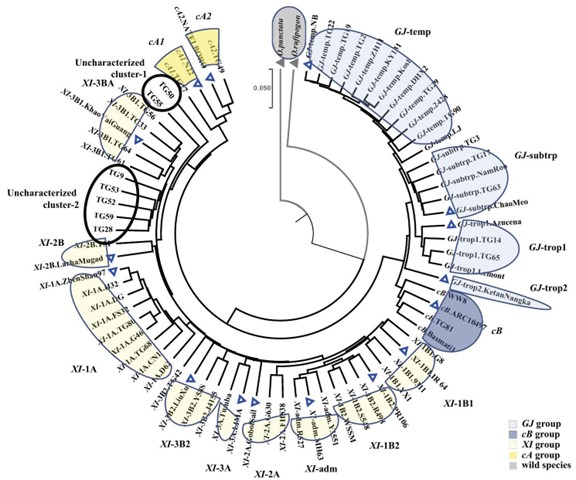
\includegraphics[width=0.8\linewidth]{figure/tree}
	\caption{使用全基因组倒位指数对75个高质量水稻基因组进行系统发育树分析} \label{tree}
\end{figure}

这部分中,研究人员使用了一些典型的数据处理方法:

\begin{enumerate}

\item UPGMA(算术平均无加权配对群组法)是一种常用的聚类方法.
它基于距离矩阵进行操作,通过计算不同样本间的成对距离,从而推断它们之间的系统发育关系.UPGMA是一种层次聚类方法,其基本思想是逐步将距离最近的样本或样本群组合并,直到所有样本都被归入一个大的群组中.


\item Mantel检验是一种数据处理方法,其计算公式如下:

$$
r=\frac{\sum_{i=1}^{n-1} \sum_{j=i+1}^n\left(X_{i j}-\bar{X}\right)\left(Y_{i j}-\bar{Y}\right)}{\sqrt{\sum_{i=1}^{n-1} \sum_{j=i+1}^n\left(X_{i j}-\bar{X}\right)^2\left(Y_{i j}-\bar{Y}\right)^2}}
$$

其中,$X_{ij}$ 和 $Y_{ij}$ 分别表示两个距离矩阵中的元素,$\bar{X}$ 和 $\bar{Y}$ 分别表示距离矩阵的平均值,$n$ 是观测值的数量.

\end{enumerate}


\subsubsection{其他分析和结果概要}
由于本报告篇幅有限,无法详细分析所有结果,以下简要概述其他部分:

\begin{enumerate}
	\item 分析了亚洲水稻及其两个野生近缘种(O. punctata和O. rufipogon)中的物种特异性、群体特异性和共享倒位.提出了特异性倒位和倒位速率的模型.
	\item 研究了水稻全基因组倒位指数中的转座子元素分布.发现三个转座子元素家族(LTR-RT Ty1-copia、Ty3-gypsy 和 DNA-TE MULE)在倒位断点处的频率较高.
	\item 分析了位于倒位断点处基因的转录丰度.展示了MH63(XI-adm)基因组中位于倒位末端的两个OsNAS基因拷贝,以及倒位对其5'UTR区域的影响.同时,研究了OsNAS基因在根组织中的转录丰度以及Fbox基因编码序列在MH63(XI-adm)中如何被倒位破坏.
	\item 对大倒位的群体连锁不平衡进行了分析.研究了倒位导致的连锁不平衡(LD)区块破坏,展示了倒位如何破坏两个LD区块.同时,给出了一个实例,说明高LD的SNP区块被倒位破坏,以及IRGSP RefSeq(GJ-temp)与Azucena(GJ-trop1)单倍型区块不连续时,INV030410区域的Azucena(GJ-trop1)单倍型区块被破坏.
\end{enumerate}

\subsubsection{基因组倒位的鉴定与评估方法}

本文的研究者旨在识别大型倒位(>100 bp),在两个基因组(GJ-temp: IRGSP-1.0 和 XIadm: MH63)上测试了四种分析流程.

工作流程1:MH63基因组切成约10倍覆盖率的50 Kb重叠片段,使用NGMLR映射到IRGSP-1.0,并用SVIM调用倒位.保留深度大于6且通过筛选标准的倒位.

工作流程2:与工作流程1类似,但使用Sniffles调用倒位.

工作流程3:MH63基因组与IRGSP-1.0使用Minimap2对齐.筛选出大于90\%同源性和长度大于100 bp的结果.使用SyRI调用倒位.

工作流程4:与工作流程3类似,但使用MUMmer的Nucmer进行对齐.

本文的研究者验证后最后选择了工作流程4,使用MUMmer将74个基因组序列与IRGSP RefSeq对齐,筛选最小90\%同源性和最小100 bp长度.用MUMmer的“showcoords”功能获取坐标.最后,使用SyRI工具调用倒位,生成包含ID、参考和查询基因组坐标起始、结束位置的VCFs,用于下游全基因组比较.

关于这部分内容,研究者开源了代码,我也尝试了在Linux系统下安装numcer,syri等软件进行序列的比对和评估测试,不过由于原文亚洲水稻基因的数据量确实比较大(一个数据集大约100多M,其实不算大,但是也不小了),暂时还没有来得及复现文章的结果,因此也不再赘述了.

\subsubsection{研究实例总结和展望}

本研究通过全面分析亚洲稻米种群结构层面的倒位变异,揭示了倒位在水稻中的重要性.倒位作为一种重要的结构变异类型,对于基因重组抑制、适应性特征选择、生殖隔离和物种形成具有显著作用.通过发现1769个非冗余倒位并估计了不同层次的倒位速率,本研究为倒位研究提供了新的见解.

展望未来,亚洲稻米泛基因组倒位指数的建立仅是揭示稻米中所有自然变异的第一步.下一步研究者将建立亚洲稻米的水稻数字基因库,将超过100,000份测序数据映射到水稻种群参考组.稻米基因组结构变异的研究和应用,将为未来稻米育种和农业发展提供支持.通过这一研究实例的学习和分析,我们也认识到泛基因组学在大规模组学数据和科学计算时代可以发挥非常重要的作用.



%\section{开始实验}
\zhlipsum[2]\cite{HPC}

计数列表环境
\begin{enumerate}
	\item 这是一个计数列表环境.
	\item 这是一个计数列表环境.
	\item 这是一个计数列表环境.
\end{enumerate}

\vspace{2ex}
不计数列表环境
\begin{itemize}
	\item 这是一个不计数列表环境.
	\item 这是一个不计数列表环境.
	\item 这是一个不计数列表环境.
\end{itemize}



一些公式:

$$
		\left\{\begin{array}{l}
			\mbox{Find } u \in X \mbox{ such that } \\
			a(u, v)=F(v),~\forall v \in X.
		\end{array} \right. 
$$
has a unique solution. Moreover, we have
\begin{equation}
	 \|u\| \leq \frac{1}{\alpha}\|F\|_{X^{\prime}}. 
\end{equation}


表格模板:

\begin{table}
	\caption{这是一个三线表.}	
	\centering
	\begin{tabular}{ccc}
		\toprule
		\textbf{Treatments} & \textbf{Response 1} & \textbf{Response 2}\\
		\midrule
		Treatment 1 & 0.0003262 & 0.562 \\
		Treatment 2 & 0.0015681 & 0.910 \\
		\bottomrule
	\end{tabular}
\end{table}


本文定义了新的可变长度左中右 (LCR) 格式, LCR 三个格式会根据表格宽度的设定自行控制宽度, 且其宽度相等, 方便设置和页面相同宽度的表格. 本文还定义了 P\{\} 格式可以设定某一列宽度 (如 P\{1cm\} 控制某一列的宽度为 1cm) 并居中.%{0.9\textwidth}
\begin{table}[!htp]
	\centering
	% PLCR已经定义
	\caption{某校学生身高体重样本.}
	\label{tab2:heightweight}	
	\begin{tabular}{lccc}
		\toprule
		序号&年龄&身高&体重\\
		\midrule
		1&14&156&42\\
		2&16&158&45\\
		3&14&162&48\\
		4&15&163&50\\
		\cmidrule{2-4}
		平均&15&159.75&46.25\\
		\bottomrule
	\end{tabular}
\end{table}

表格示例
%\begin{table}[htp!]
%	\centering
%	\renewcommand\arraystretch{1.2} %定义表格高度
%	% PLCR前面已经定义
%	\caption{表格的描述.}
%	\label{tab3:NumError}
%	\begin{tabularx}{0.9\textwidth}{|P{1cm}|c|c|c|c|}
%		\Xhline{2\arrayrulewidth}
%		N  & A       & B    & C  & D   \\
%		\Xhline{2\arrayrulewidth}
%		1  & 9.20E-05 & 9.90E-05 & 1.00E-06 & 8.00E-06  \\
%		2  & 9.80E-05 & 8.00E-05 & 7.00E-06 & 1.40E-05  \\
%		3  & 4.00E-06 & 8.10E-05 & 8.80E-05 & 2.00E-05 \\
%		4  & 8.50E-05 & 8.70E-05 & 1.90E-05 & 2.10E-05 \\
%		5 & 8.60E-05 & 9.30E-05 & 2.50E-05 & 2.00E-06  \\
%		6 & 1.70E-05 & 2.40E-05 & 7.60E-05 & 8.30E-05  \\
%		7 & 2.30E-05 & 5.00E-06 & 8.20E-05 & 8.90E-05 \\
%		8 & 7.90E-05 & 6.00E-06 & 1.30E-05 & 9.50E-05  \\
%		9 & 1.00E-05 & 1.20E-05 & 9.40E-05 & 9.60E-05 \\
%		\Xhline{2\arrayrulewidth}
%	\end{tabularx}
%\end{table}


\begin{lstlisting}[caption = cs代码表测试]
	import keras
	from keras import layers
	
	def train_model(maxword, maxlen):
	model = keras.Sequential()
	
	# 前面数据需要的“词向量化”的操作,不算双向RNN的要求:
	model.add( layers.Embedding(maxword, 50, input_length=maxlen) )
	
	# 双向RNN搭建:
	model.add( layers.Bidirectional( layers.LSTM(64, dropout = 0.2, recurrent_dropout = 0.5) ) )
	
	# 外接一个单独的dropout层:非必须
	model.add( layers.Dropout(0.2) )
	
	# 进入全连接层:二分类,1个神经元就够
	model.add( layers.Dense(1, activation='sigmoid') )
	
	# 网络编译也在这个函数内完成:内容没变化
	model.compile( optimizer='adam',
	loss = 'binary_crossentropy',
	metrics = ['acc']
	) 
	return model
\end{lstlisting}

%\section{实验结果分析}
\zhlipsum[3]

Uncomment the code on this slide to include your own image from the same directory as the template .TeX file.
\begin{figure}[htp!]
	\centering
	\includegraphics[width=0.5\linewidth]{figure/image1}
	\caption{图的描述.} \label{fig:A}
\end{figure}


\begin{figure}[htb]
	\centering
	\begin{minipage}{0.48\linewidth}
		\centering
		\includegraphics[width=\linewidth]{figure/image1}
		\caption{图~1~的描述.}
	\end{minipage}\hfill
	\begin{minipage}{0.48\linewidth}
		\centering
		\includegraphics[width=\linewidth]{figure/image2}
		\caption{图~2~的描述.}
	\end{minipage}
\end{figure}

%\newpage
%\thispagestyle{IEEEtran}
%\bibliographystyle{plainnat}
\bibliography{books}
%\newpage

\appendix

%\section{串行部分全部实验结果}

图或者代码放上来。

\section{并行部分全部实验结果}

图或者代码放上来。

\end{document}